\section{Case Study}

In this example we explore the auto-transplantation of content within the "bosses" of the video game Kromaia.

\textbf{Metamodel definition}

First, a simplified example from the game metamodel (Fig.~\ref{fig:metamodel}, the concret syntax of the model (Fig.~\ref{fig:syntax} from the video game Kromaia. In this example we use a graphical representation to help the comprehension of the reader. It is not neccesary to use a graphic model representation. The type of model will depend on the metamodel and models that developers are used to.


\begin{figure}[h]
    \centering
    \includegraphics[width=0.45\textwidth]{Figures/metamodel.png}
    \caption{Simplified metamodel}
    \label{fig:metamodel}
\end{figure}

\begin{figure}[h]
    \centering
    \includegraphics[width=0.45\textwidth]{Figures/syntaxmodel.png}
    \caption{Concrete syntax of the model}
    \label{fig:syntax}
\end{figure}

\textbf{Features selection}

From the models of the content, developers will select a source model content (donor), a target model content (host) and the organ that will be transplanted. 

The donor is a simplified version of an original "boss" from Kromaia, called "Serpent" (Fig.~\ref{fig:donor}. The original model is a XML with approximatly 1700 lines of code.

The host is a regular enemy on Kromaia (Fig.~\ref{fig:host}.

\begin{figure}[h]
    \centering
    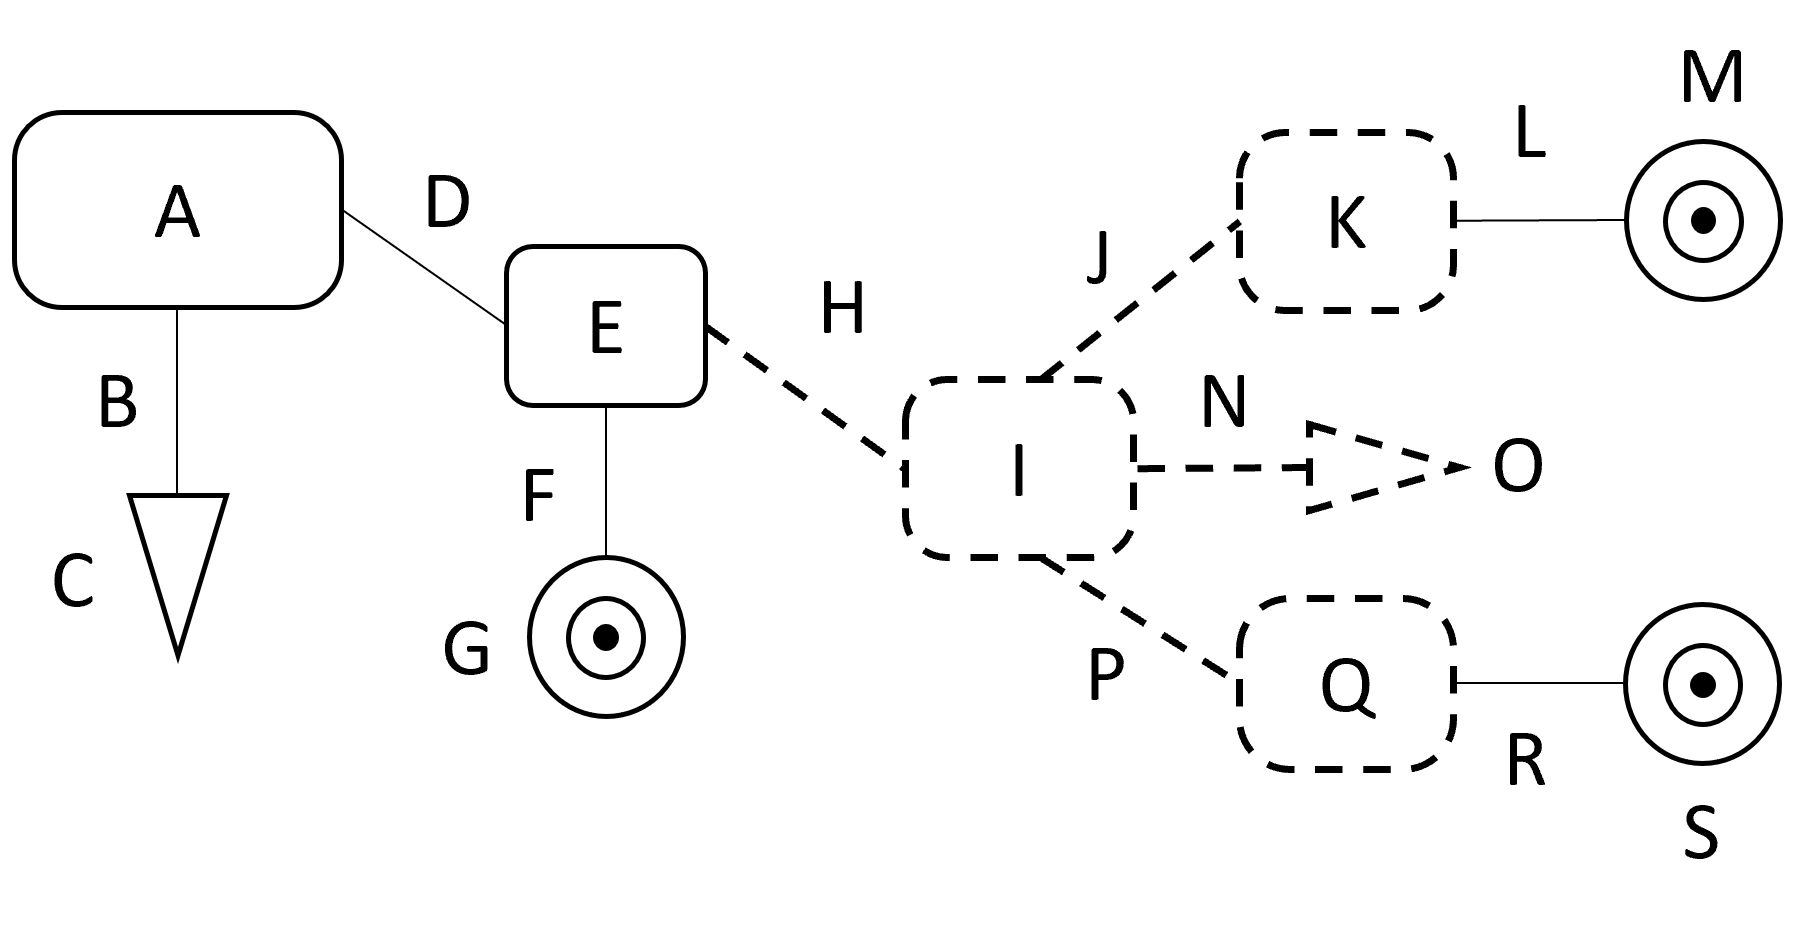
\includegraphics[width=0.45\textwidth]{Figures/donor+organ.png}
    \caption{Donor with organ selection in green. The letters represent each element of the model.}
    \label{fig:donor}
\end{figure}

\begin{figure}[h]
    \centering
    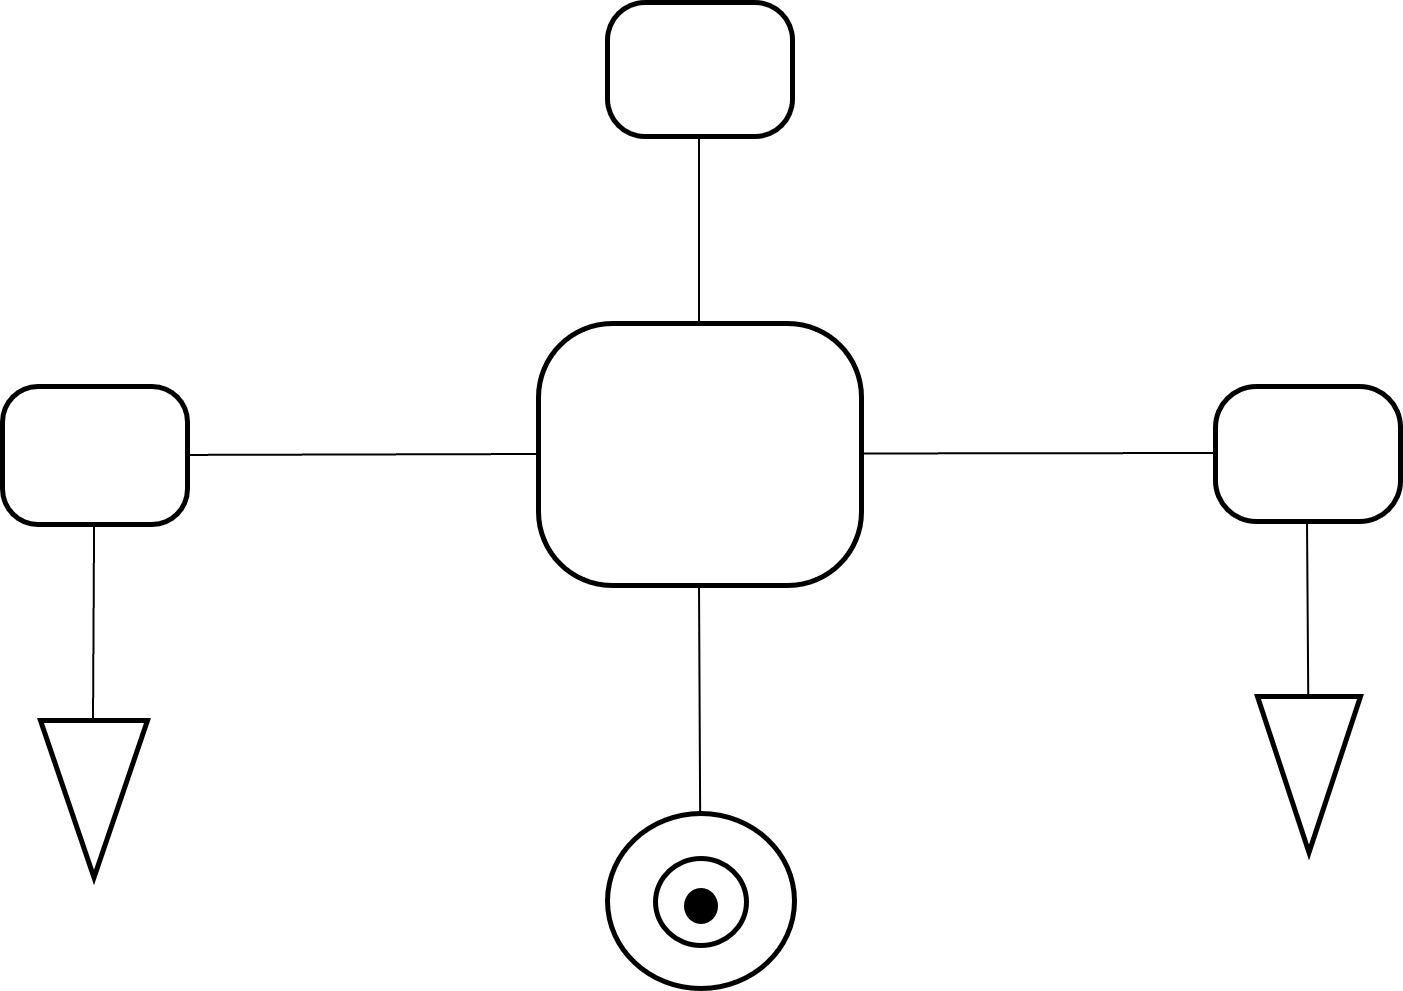
\includegraphics[width=0.3\textwidth]{Figures/host.png}
    \caption{Host}
    \label{fig:host}
\end{figure}

\textbf{Organ boundaries}

The approach based on the restrictions of the metamodel, the donor, and the selected elements of the organ (H, I, J, K, L, N, O, P, Q) will define the boundaries of the organ to be transplantated. The boundaries are the connections that the selected organ has with the rest of the donor. The elements that connect with the rest of the donor are H, K, and Q, so we will have a boundary on each element. Fig.~\ref{fig:org_bound} shows the boundary of element H as b11, K as b16, and Q, as b25.

\begin{figure}[h]
    \centering
    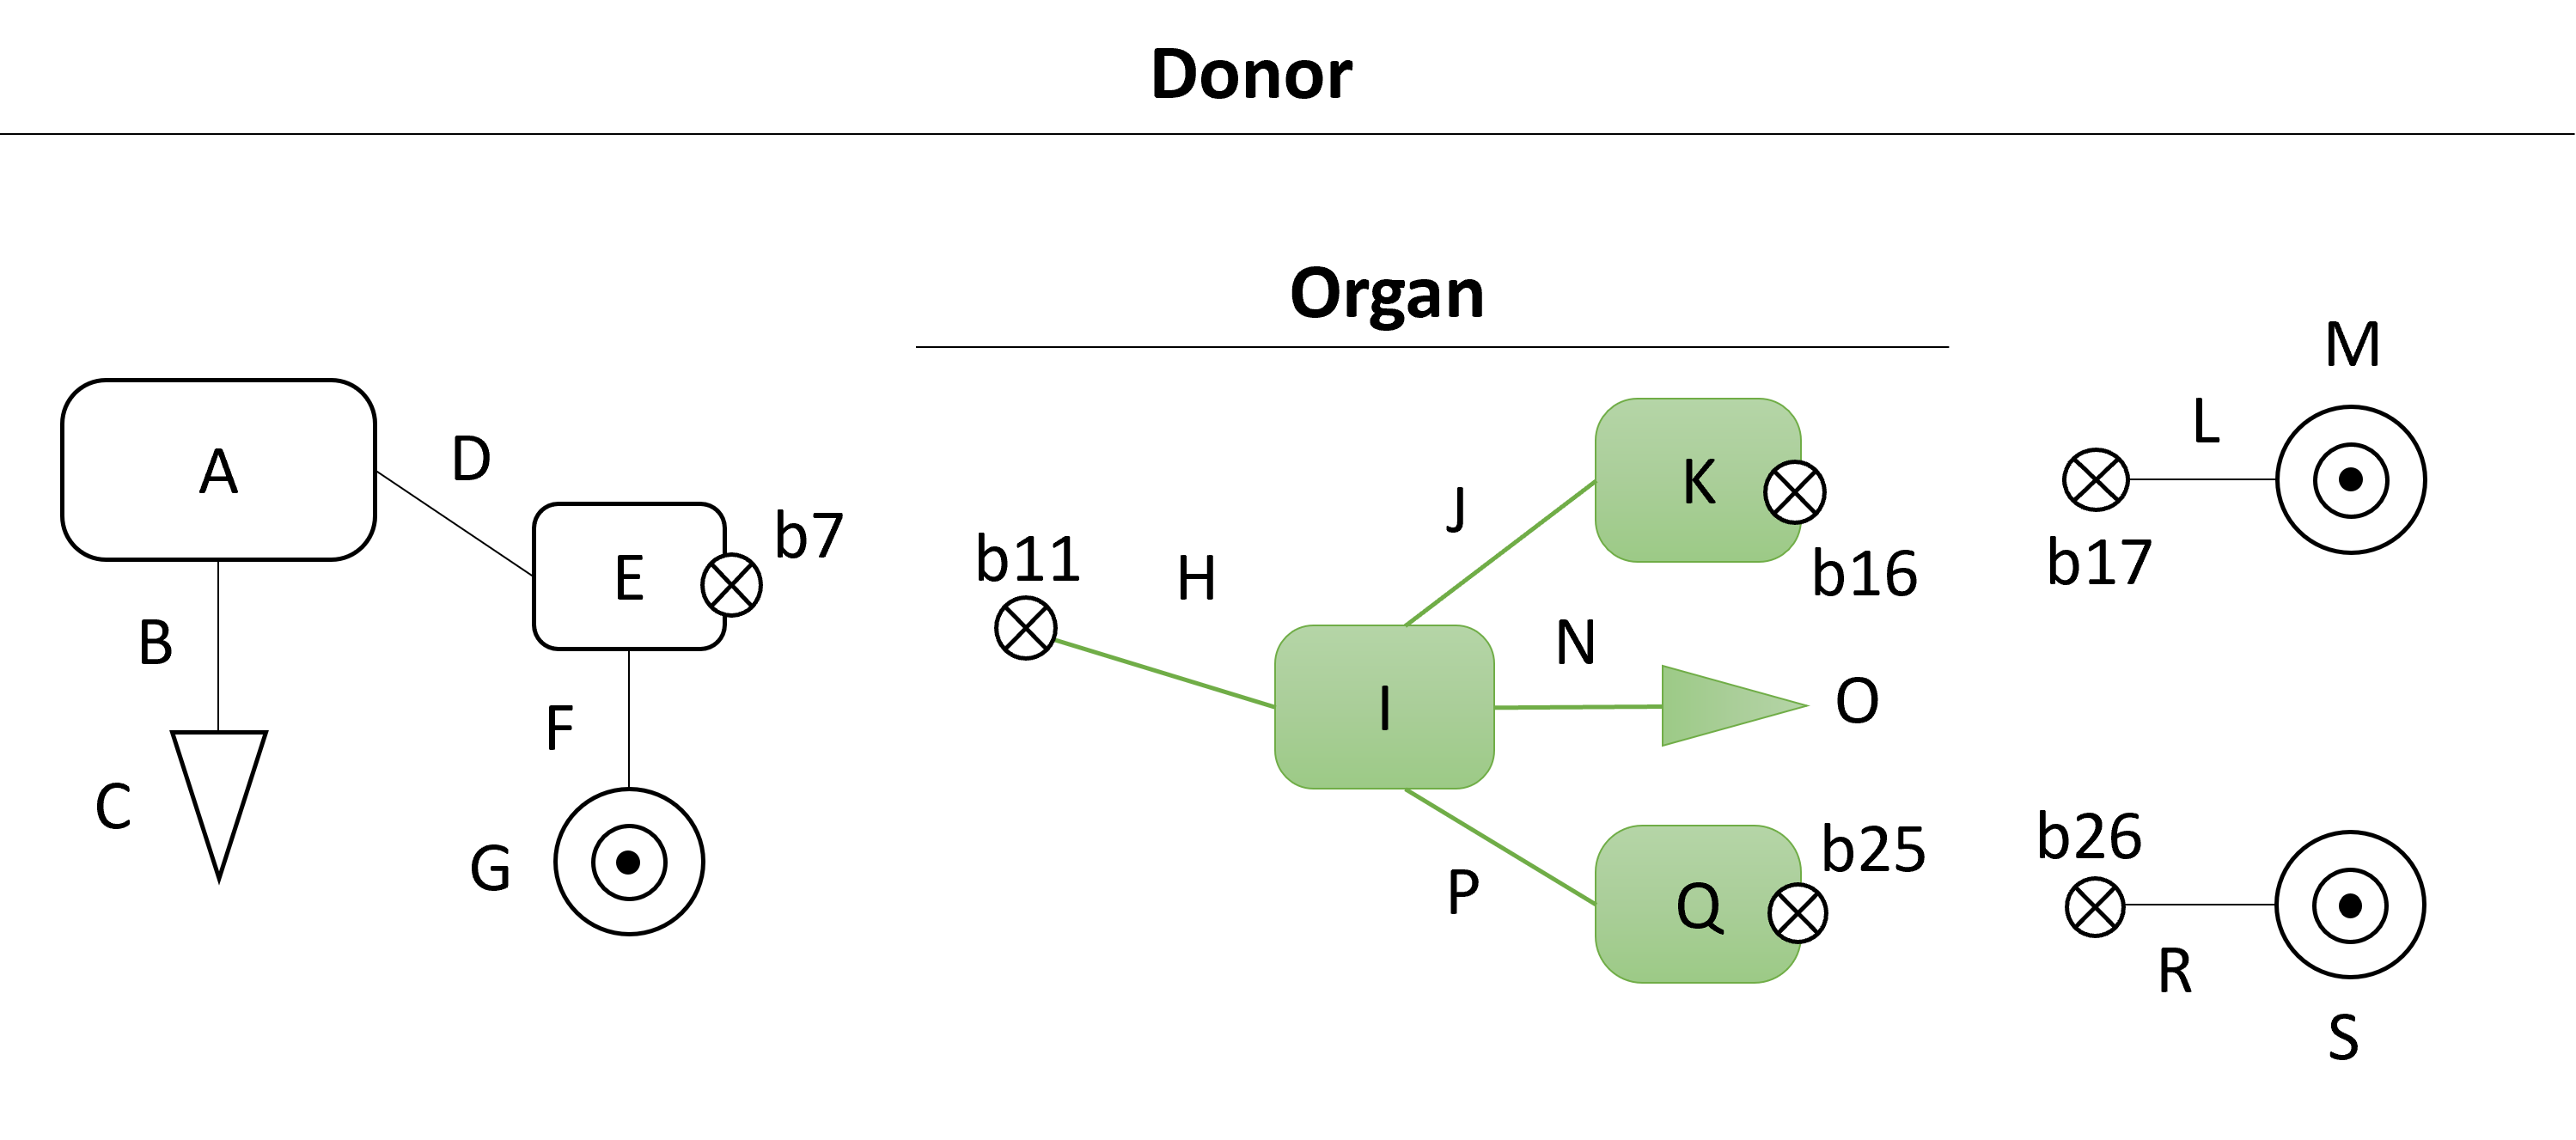
\includegraphics[width=0.45\textwidth]{Figures/donor+organ_boundaries.png}
    \caption{Definition of organ boundaries. The boundary is represented by a circle crosed.}
    \label{fig:org_bound}
\end{figure}

\textbf{Boundaries mapping}

Then we need to all possible compatible boundaries between the organ and the host.

- For each element in the host the approach define its boundaries (Fig.\ref{fig:host_bound}.

- From each boundary in the organ we map the all possible compatibilities with host boundaries, including the possibility of not connecting the boundary to the host boundaries (Table.~\ref{tab:boundaries}.

% Please add the following required packages to your document preamble:
% \usepackage{multirow}
% \usepackage[table,xcdraw]{xcolor}
% If you use beamer only pass "xcolor=table" option, i.e. \documentclass[xcolor=table]{beamer}
\begin{table}[]
\begin{tabular}{|c|ll|}
\hline
{\color[HTML]{000000} Organ boundary}                                     & \multicolumn{2}{c|}{{\color[HTML]{000000} \begin{tabular}[c]{@{}c@{}}Host \\      boundaries\end{tabular}}} \\ \hline
                                                                          & \multicolumn{1}{c|}{ba}                         & \multicolumn{1}{c|}{bm}                                   \\ \cline{2-3} 
                                                                          & \multicolumn{1}{c|}{bd}                         & \multicolumn{1}{c|}{bp}                                   \\ \cline{2-3} 
                                                                          & \multicolumn{1}{c|}{bg}                         & \multicolumn{1}{c|}{Bs}                                   \\ \cline{2-3} 
\multirow{-4}{*}{b11}                                                     & \multicolumn{1}{c|}{bj}                         & \multicolumn{1}{c|}{Not connected}                        \\ \hline
                                                                          & \multicolumn{1}{l|}{bb}                         & bc                                                        \\ \cline{2-3} 
                                                                          & \multicolumn{1}{l|}{be}                         & bf                                                        \\ \cline{2-3} 
                                                                          & \multicolumn{1}{l|}{bh}                         & bi                                                        \\ \cline{2-3} 
                                                                          & \multicolumn{1}{l|}{bk}                         & bl                                                        \\ \cline{2-3} 
                                                                          & \multicolumn{1}{l|}{bn}                         & bo                                                        \\ \cline{2-3} 
\multirow{-6}{*}{\begin{tabular}[c]{@{}c@{}}b16\\    \\ b25\end{tabular}} & \multicolumn{2}{l|}{Not connected}                                                                          \\ \hline
\end{tabular}
\caption{Mapping  of compatible boundaries between organ and host}
\label{tab:boundaries}
\end{table}

\begin{figure}[h]
    \centering
    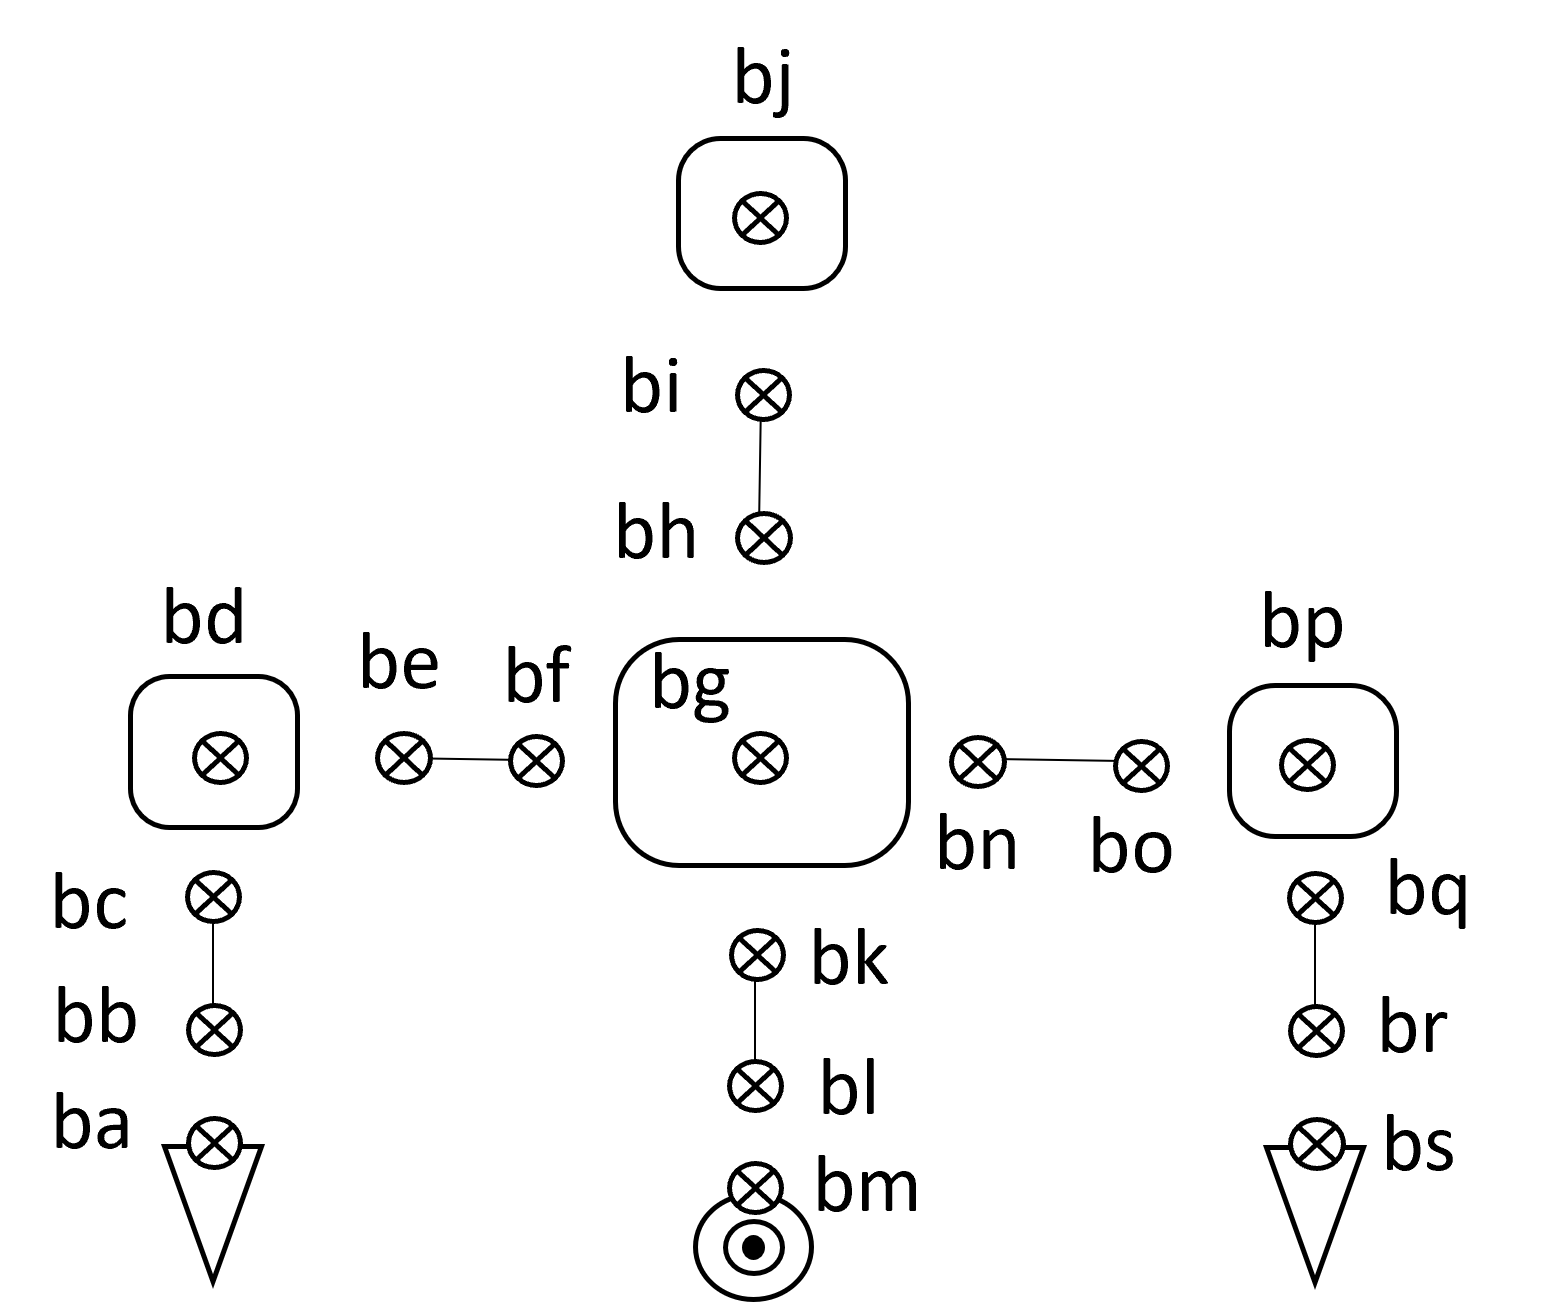
\includegraphics[width=0.45\textwidth]{Figures/host_boundaries.png}
    \caption{Definition of host boundaries. The boundary is represented by a circle crosed.}
    \label{fig:host_bound}
\end{figure}

\textbf{Operations}

The selection operator will use the boundaries donor + organ mapping to define the connection between the organ and the donor.

Here comes mutation and crossover operators creating a new candidates. Different possible results handmaded are presented in Figure.~\ref{fig:candidates}

\textbf{Objective function}

New candidates are evaluated by the objective function through simulation. In classical software engineering is common to use test cases in the objective function~\cite{}. However, in video games research field other type of evaluation in the objective function such as simulations are commonly used~\cite{}.

\begin{figure}[h]
    \centering
    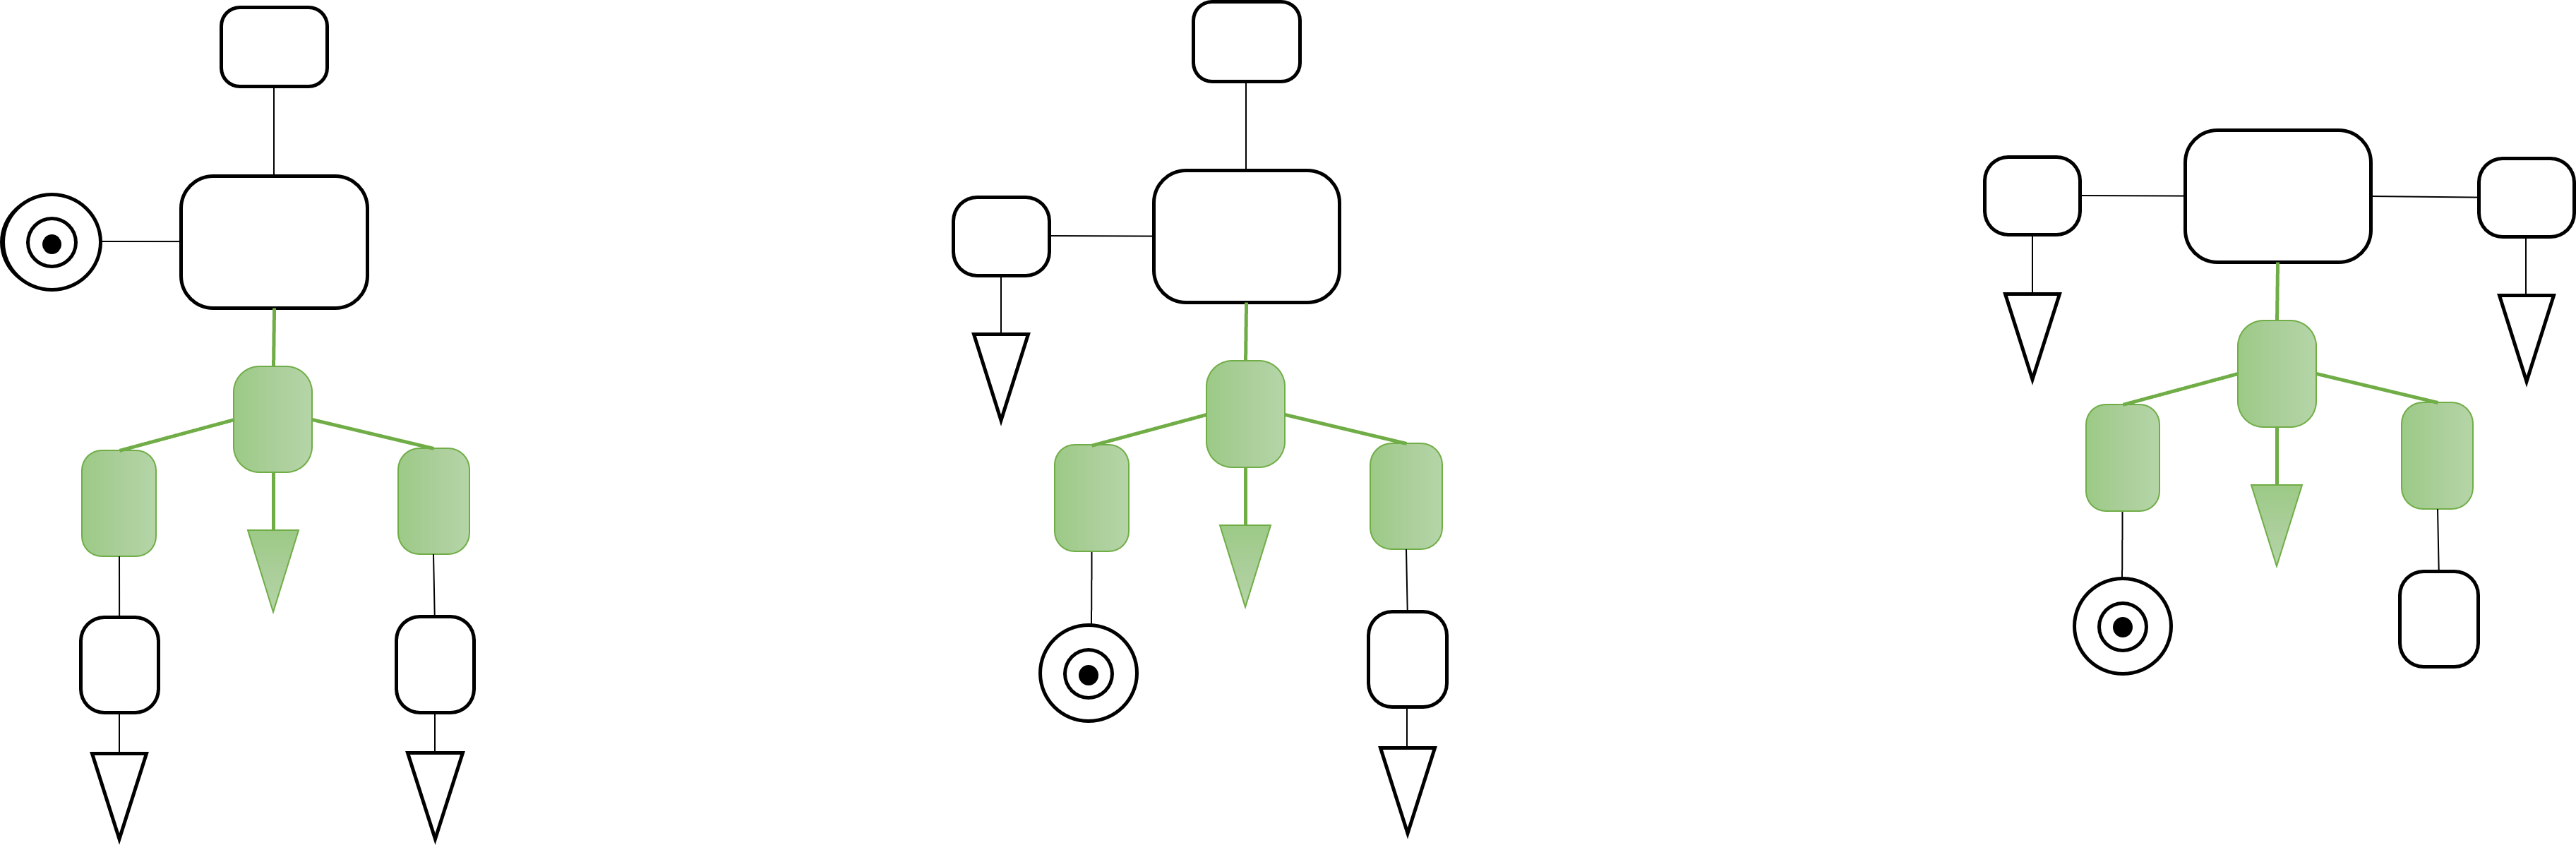
\includegraphics[width=0.45\textwidth]{Figures/candidates.png}
    \caption{Population candidates to be evaluated}
    \label{fig:candidates}
\end{figure}

\subsection{Encoding}





\subsection{Objective Function}

The objective function in \ApproachName{} assess the quality of each individual as a model. This is done by two means; Test-based and Simulation-based objective functions. The state-of-the-art in software transplantation mainly work with Test-based objective function. From the state-of-the-art in video games software there is a lot of work with Simulation-based objective function.

For the Test-based objective function the developers from \CaseStudy{} provided us a total of 243 test selected under they domain knowledge. \mar{more info about test?}

When applying \ApproachName{} to the \CaseStudy{} case study, the validity of the models is performed by a run-time interpreter that is part of the game. \mar{do we go through the validity too?}

When no validation errors are found for a certain boss model and it is confirmed as valid, its fitness value is obtained from a simulation that reproduces a duel between the boss of the model and a human player. 

During that simulation, the player faces the boss in order to destroy the weak points that are available at that moment, whereas the boss acts according to the anatomy, behaviour, and attack/defense balance that is included in its model, trying to defeat the player. In that simulation, both the boss and the human player try to win the match and do not avoid confrontation, try to prevent draw/tie games, and try to ensure that there is a winner. The objective value is calculated once the simulation process is finished, and our approach collects information on the battle progress and key events.

The information retrieved from the simulation is the data that the developers regard as relevant, using their domain knowledge, for determining whether or not a boss is suitable for a commercial release of the video game, i.e., the percentage of human player victories ($F_{Victory}$) and the percentage of human player health left once the player wins a duel ($F_{Health}$). The $clamp$ function is used in the fitness measures:

\begin{equation}
clamp_{[0, 1]}( x ) = max ( 0, min ( x, 1 ) )
\end{equation}

In our approach, $F_{Victory}$ is calculated as a measure of the difference between the number of human player victories ($V_{P}$) and the optimal number of victories (33\%, according to the developers of \CaseStudy{} and their criteria) ($V_{Optimal}$):
\begin{equation}
F_{Victory} = clamp_{[0, 1]} \left ( 1 -\frac{\mid V_{Optimal} - V_{P} \mid}{ V_{Optimal}} \right )
\end{equation}

The criterion $F_{Health}$, which refers to completed duels that end in human player victories, is the average difference between the human player's health percentage once the duel is over ($\Theta_{P}$) and the optimal health level that the player should have at that point ($\Theta_{Optimal}$, 20\%, according to the developers):
\begin{equation}
F_{Health} = clamp_{[0, 1]} \left ( 1 - \frac{\sum\limits_{d=1}^{V_{P}}\frac{\mid \Theta_{Optimal} - \Theta_{P} \mid}{ \Theta_{Optimal}}}{V_{P}} \right )
\end{equation}

$F_{Overall}$ is an average fitness value for a boss model that includes the fitness criteria described above and validation information, with $Validity$ being a value that determines whether or not a model is valid (1 and 0, respectively):
\begin{equation}
F_{Overall} = min( Validity, \frac{\sum\limits_{i=1}^{N}F_{i}}{N} )
\end{equation}

In the end, $F_{Overall}$ is a value in [0, 1] that is used to assess a boss model when our \ApproachName{} approach is applied to the \CaseStudy{} case study.

